% =====================================================================
% 6. Final comparison, critical discussion and conclusions
% =====================================================================
\section{Final comparison and critical discussion}\label{sec:discussion}

\subsection{All final models}

Table~\ref{tab:comparison_final} and Figure~\ref{fig:comparison_overview} collect every final model of
the three areas on the test fold (shared task T15).

% Shared float (common/make_floats.py). Table: tables/comparison_final.tex
\begin{table}[htbp]
\centering
\caption[Final comparison (test)]{Final comparison on the test fold. Mean $\pm$ SD over seeds; interval: 95\,\% patient bootstrap of the first seed. Published rows: macro AUC of the superclass task in Table~I of \cite{strodthoff2021deep}, obtained in a different setting (described in the text).}
\label{tab:comparison_final}
\small
\begin{adjustbox}{max width=\textwidth}
% Generated by src/comparison.py from results/logs/comparison_summary.json.
% Mean +- SD over seeds (one run: no SD); CI = 95% patient bootstrap of the first seed. Needs alias "comparison".
\begin{tabular}{lcrrccc}
\toprule
Model & Labels & Train.\ param. & Seeds & Test macro AUROC & First seed [95\% CI] & Test macro F1 \\
\midrule
\multicolumn{7}{l}{\textit{12 leads}} \\
\quad Trivial (lead mean and SD) & 100\% & \comparisonParamsTrivial{} & \comparisonNSeedsTrivial{} & \comparisonTestAurocMeanTrivial{} & \comparisonTestAurocFirstTrivial{} [\comparisonTestAurocLoFirstTrivial{}, \comparisonTestAurocHiFirstTrivial{}] & \comparisonTestFOneMeanTrivial{} \\
\quad Dense & 100\% & \comparisonParamsTwelveDense{} & \comparisonNSeedsTwelveDense{} & \comparisonTestAurocMeanTwelveDense{} $\pm$ \comparisonTestAurocSdTwelveDense{} & \comparisonTestAurocFirstTwelveDense{} [\comparisonTestAurocLoFirstTwelveDense{}, \comparisonTestAurocHiFirstTwelveDense{}] & \comparisonTestFOneMeanTwelveDense{} $\pm$ \comparisonTestFOneSdTwelveDense{} \\
\quad CNN & 100\% & \comparisonParamsTwelveCnn{} & \comparisonNSeedsTwelveCnn{} & \comparisonTestAurocMeanTwelveCnn{} $\pm$ \comparisonTestAurocSdTwelveCnn{} & \comparisonTestAurocFirstTwelveCnn{} [\comparisonTestAurocLoFirstTwelveCnn{}, \comparisonTestAurocHiFirstTwelveCnn{}] & \comparisonTestFOneMeanTwelveCnn{} $\pm$ \comparisonTestFOneSdTwelveCnn{} \\
\quad RNN & 100\% & \comparisonParamsTwelveRnn{} & \comparisonNSeedsTwelveRnn{} & \comparisonTestAurocMeanTwelveRnn{} $\pm$ \comparisonTestAurocSdTwelveRnn{} & \comparisonTestAurocFirstTwelveRnn{} [\comparisonTestAurocLoFirstTwelveRnn{}, \comparisonTestAurocHiFirstTwelveRnn{}] & \comparisonTestFOneMeanTwelveRnn{} $\pm$ \comparisonTestFOneSdTwelveRnn{} \\
\quad RNN + attention & 100\% & \comparisonParamsTwelveRnnattn{} & \comparisonNSeedsTwelveRnnattn{} & \comparisonTestAurocMeanTwelveRnnattn{} $\pm$ \comparisonTestAurocSdTwelveRnnattn{} & \comparisonTestAurocFirstTwelveRnnattn{} [\comparisonTestAurocLoFirstTwelveRnnattn{}, \comparisonTestAurocHiFirstTwelveRnnattn{}] & \comparisonTestFOneMeanTwelveRnnattn{} $\pm$ \comparisonTestFOneSdTwelveRnnattn{} \\
\quad Transformer & 100\% & \comparisonParamsTwelveTransformer{} & \comparisonNSeedsTwelveTransformer{} & \comparisonTestAurocMeanTwelveTransformer{} $\pm$ \comparisonTestAurocSdTwelveTransformer{} & \comparisonTestAurocFirstTwelveTransformer{} [\comparisonTestAurocLoFirstTwelveTransformer{}, \comparisonTestAurocHiFirstTwelveTransformer{}] & \comparisonTestFOneMeanTwelveTransformer{} $\pm$ \comparisonTestFOneSdTwelveTransformer{} \\
\addlinespace
\multicolumn{7}{l}{\textit{Lead II only (T14)}} \\
\quad Dense & 100\% & \comparisonParamsOneleadDense{} & \comparisonNSeedsOneleadDense{} & \comparisonTestAurocMeanOneleadDense{} $\pm$ \comparisonTestAurocSdOneleadDense{} & \comparisonTestAurocFirstOneleadDense{} [\comparisonTestAurocLoFirstOneleadDense{}, \comparisonTestAurocHiFirstOneleadDense{}] & \comparisonTestFOneMeanOneleadDense{} $\pm$ \comparisonTestFOneSdOneleadDense{} \\
\quad CNN & 100\% & \comparisonParamsOneleadCnn{} & \comparisonNSeedsOneleadCnn{} & \comparisonTestAurocMeanOneleadCnn{} $\pm$ \comparisonTestAurocSdOneleadCnn{} & \comparisonTestAurocFirstOneleadCnn{} [\comparisonTestAurocLoFirstOneleadCnn{}, \comparisonTestAurocHiFirstOneleadCnn{}] & \comparisonTestFOneMeanOneleadCnn{} $\pm$ \comparisonTestFOneSdOneleadCnn{} \\
\quad RNN & 100\% & \comparisonParamsOneleadRnn{} & \comparisonNSeedsOneleadRnn{} & \comparisonTestAurocMeanOneleadRnn{} $\pm$ \comparisonTestAurocSdOneleadRnn{} & \comparisonTestAurocFirstOneleadRnn{} [\comparisonTestAurocLoFirstOneleadRnn{}, \comparisonTestAurocHiFirstOneleadRnn{}] & \comparisonTestFOneMeanOneleadRnn{} $\pm$ \comparisonTestFOneSdOneleadRnn{} \\
\quad RNN + attention & 100\% & \comparisonParamsOneleadRnnattn{} & \comparisonNSeedsOneleadRnnattn{} & \comparisonTestAurocMeanOneleadRnnattn{} $\pm$ \comparisonTestAurocSdOneleadRnnattn{} & \comparisonTestAurocFirstOneleadRnnattn{} [\comparisonTestAurocLoFirstOneleadRnnattn{}, \comparisonTestAurocHiFirstOneleadRnnattn{}] & \comparisonTestFOneMeanOneleadRnnattn{} $\pm$ \comparisonTestFOneSdOneleadRnnattn{} \\
\quad Transformer & 100\% & \comparisonParamsOneleadTransformer{} & \comparisonNSeedsOneleadTransformer{} & \comparisonTestAurocMeanOneleadTransformer{} $\pm$ \comparisonTestAurocSdOneleadTransformer{} & \comparisonTestAurocFirstOneleadTransformer{} [\comparisonTestAurocLoFirstOneleadTransformer{}, \comparisonTestAurocHiFirstOneleadTransformer{}] & \comparisonTestFOneMeanOneleadTransformer{} $\pm$ \comparisonTestFOneSdOneleadTransformer{} \\
\addlinespace
\multicolumn{7}{l}{\textit{Lead II, ECG-GPT transfer (T13)}} \\
\quad ECG-GPT, from scratch & 100\% & \comparisonParamsScratchFOneZeroZero{} & \comparisonNSeedsScratchFOneZeroZero{} & \comparisonTestAurocMeanScratchFOneZeroZero{} $\pm$ \comparisonTestAurocSdScratchFOneZeroZero{} & \comparisonTestAurocFirstScratchFOneZeroZero{} [\comparisonTestAurocLoFirstScratchFOneZeroZero{}, \comparisonTestAurocHiFirstScratchFOneZeroZero{}] & \comparisonTestFOneMeanScratchFOneZeroZero{} $\pm$ \comparisonTestFOneSdScratchFOneZeroZero{} \\
\quad ECG-GPT, linear probe (frozen) & 100\% & \comparisonParamsProbeFOneZeroZero{} & \comparisonNSeedsProbeFOneZeroZero{} & \comparisonTestAurocMeanProbeFOneZeroZero{} $\pm$ \comparisonTestAurocSdProbeFOneZeroZero{} & \comparisonTestAurocFirstProbeFOneZeroZero{} [\comparisonTestAurocLoFirstProbeFOneZeroZero{}, \comparisonTestAurocHiFirstProbeFOneZeroZero{}] & \comparisonTestFOneMeanProbeFOneZeroZero{} $\pm$ \comparisonTestFOneSdProbeFOneZeroZero{} \\
\quad ECG-GPT, fine-tuning & 100\% & \comparisonParamsFinetuneFOneZeroZero{} & \comparisonNSeedsFinetuneFOneZeroZero{} & \comparisonTestAurocMeanFinetuneFOneZeroZero{} $\pm$ \comparisonTestAurocSdFinetuneFOneZeroZero{} & \comparisonTestAurocFirstFinetuneFOneZeroZero{} [\comparisonTestAurocLoFirstFinetuneFOneZeroZero{}, \comparisonTestAurocHiFirstFinetuneFOneZeroZero{}] & \comparisonTestFOneMeanFinetuneFOneZeroZero{} $\pm$ \comparisonTestFOneSdFinetuneFOneZeroZero{} \\
\quad ECG-GPT, from scratch & 10\% & \comparisonParamsScratchFOneZero{} & \comparisonNSeedsScratchFOneZero{} & \comparisonTestAurocMeanScratchFOneZero{} $\pm$ \comparisonTestAurocSdScratchFOneZero{} & \comparisonTestAurocFirstScratchFOneZero{} [\comparisonTestAurocLoFirstScratchFOneZero{}, \comparisonTestAurocHiFirstScratchFOneZero{}] & \comparisonTestFOneMeanScratchFOneZero{} $\pm$ \comparisonTestFOneSdScratchFOneZero{} \\
\quad ECG-GPT, linear probe (frozen) & 10\% & \comparisonParamsProbeFOneZero{} & \comparisonNSeedsProbeFOneZero{} & \comparisonTestAurocMeanProbeFOneZero{} $\pm$ \comparisonTestAurocSdProbeFOneZero{} & \comparisonTestAurocFirstProbeFOneZero{} [\comparisonTestAurocLoFirstProbeFOneZero{}, \comparisonTestAurocHiFirstProbeFOneZero{}] & \comparisonTestFOneMeanProbeFOneZero{} $\pm$ \comparisonTestFOneSdProbeFOneZero{} \\
\quad ECG-GPT, fine-tuning & 10\% & \comparisonParamsFinetuneFOneZero{} & \comparisonNSeedsFinetuneFOneZero{} & \comparisonTestAurocMeanFinetuneFOneZero{} $\pm$ \comparisonTestAurocSdFinetuneFOneZero{} & \comparisonTestAurocFirstFinetuneFOneZero{} [\comparisonTestAurocLoFirstFinetuneFOneZero{}, \comparisonTestAurocHiFirstFinetuneFOneZero{}] & \comparisonTestFOneMeanFinetuneFOneZero{} $\pm$ \comparisonTestFOneSdFinetuneFOneZero{} \\
\addlinespace
\multicolumn{7}{l}{\textit{Lead II, zero-shot (T24)}} \\
\quad CLIP ViT-B/32, zero-shot & 0\% & --- & \comparisonNSeedsZeroshot{} & \comparisonTestAurocMeanZeroshot{} & \comparisonTestAurocFirstZeroshot{} [\comparisonTestAurocLoFirstZeroshot{}, \comparisonTestAurocHiFirstZeroshot{}] & \comparisonTestFOneMeanZeroshot{} \\
\addlinespace
\multicolumn{7}{l}{\textit{Published (quoted, different settings: see text)}} \\
\quad resnet1d\_wang, 12 leads~\cite{strodthoff2021deep} & & & & \comparisonPublishedStrodthoffResnetOneDWang{} & & \\
\quad xresnet1d101, 12 leads~\cite{strodthoff2021deep} & & & & \comparisonPublishedStrodthoffXresnetOneDOneZeroOne{} & & \\
\quad lstm, 12 leads~\cite{strodthoff2021deep} & & & & \comparisonPublishedStrodthoffLstm{} & & \\
\quad fcn\_wang, 12 leads~\cite{strodthoff2021deep} & & & & \comparisonPublishedStrodthoffFcnWang{} & & \\
\quad inception1d, 12 leads~\cite{strodthoff2021deep} & & & & \comparisonPublishedStrodthoffInceptionOneD{} & & \\
\quad lstm\_bidir, 12 leads~\cite{strodthoff2021deep} & & & & \comparisonPublishedStrodthoffLstmBidir{} & & \\
\quad Wavelet+NN, 12 leads~\cite{strodthoff2021deep} & & & & \comparisonPublishedStrodthoffWaveletNn{} & & \\
\quad ensemble, 12 leads~\cite{strodthoff2021deep} & & & & \comparisonPublishedStrodthoffEnsemble{} & & \\
\bottomrule
\end{tabular}

\end{adjustbox}
\end{table}

% Shared float (common/make_floats.py). Figure: figures/comparison_overview.pdf
\begin{figure}[htbp]
\centering
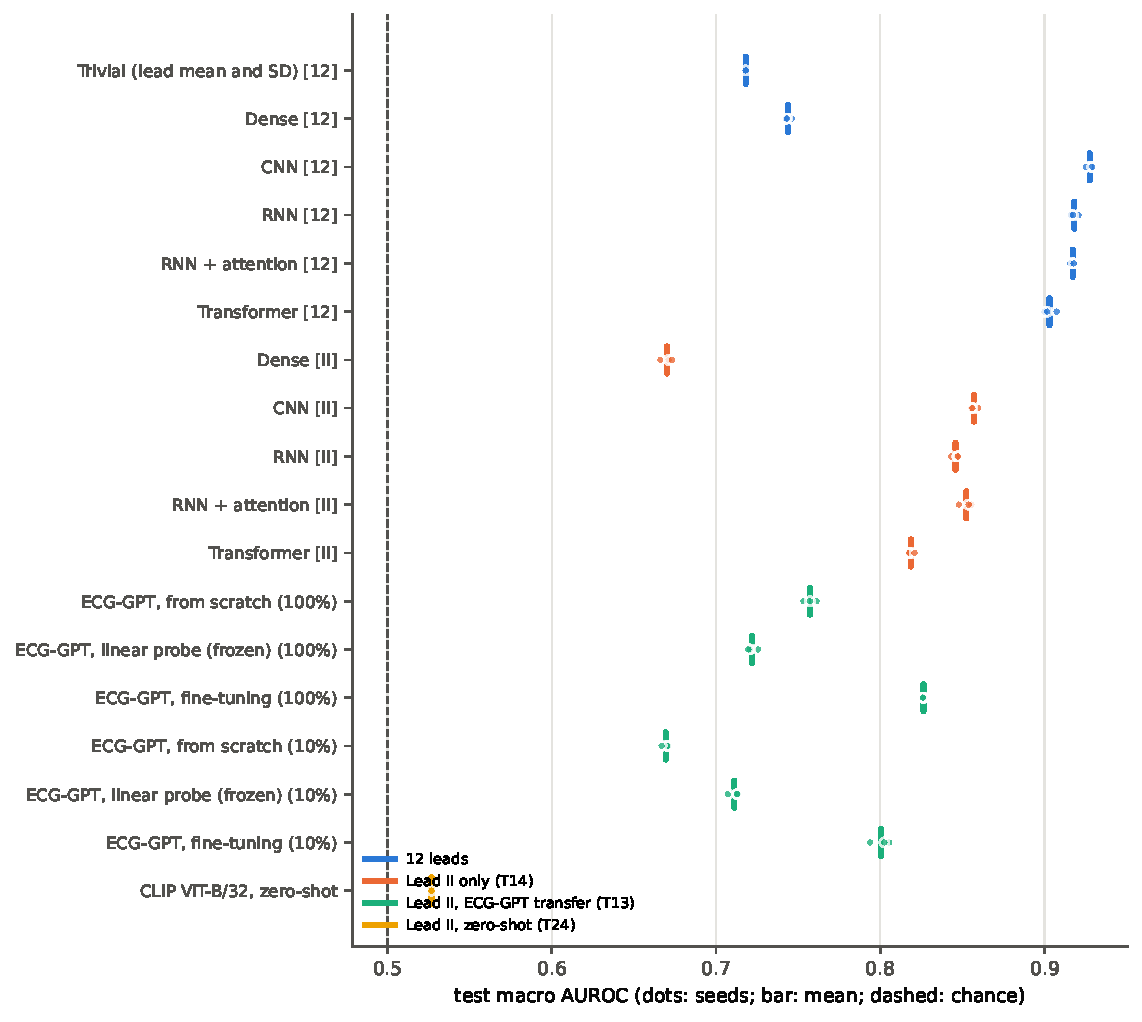
\includegraphics[width=\textwidth,height=0.42\textheight,keepaspectratio]{figures/comparison_overview.pdf}
\caption[All final models on the test fold]{Every final model on the test fold: macro AUROC (dots: seeds; bar: mean; dashed: chance). Blue: 12 leads; orange: lead II; green: ECG-GPT transfer (lead II); yellow: zero-shot CLIP (lead II images).}
\label{fig:comparison_overview}
\end{figure}


\subsection{Published results}\label{sec:published}

The published rows are the macro AUC of the superclass task in Table~I of Strodthoff et al.\
\cite[p.~1523]{strodthoff2021deep} (journal version), and they come from a different setting, which we
describe rather than adjust. Like us, they use the recommended folds, the 100\,Hz signals and the
records with at least one label of the task \cite[pp.~1520--1523]{strodthoff2021deep}. Unlike us, they
train on windows of 2.5\,s whose predictions are ``aggregated using the element-wise maximum'', with
``1-cycle learning rate scheduling \ldots\ and the AdamW optimizer'' \cite[p.~1521]{strodthoff2021deep};
each value is one model, not a mean over three seeds, and the number in brackets of their table gives
the bootstrap interval as a deviation from the point estimate (``0.743(09) is supposed to be understood as
0.743 $\pm$ 0.009'' \cite[p.~1522]{strodthoff2021deep}), not a standard deviation over seeds. With these differences in mind, our best model (the 12-lead CNN,
\comparisonTestAurocMeanTwelveCnn{}) is at the level of their best single model
(\comparisonPublishedStrodthoffResnetOneDWang{}); in their study ``only in the super-diagnostic case the
ensemble outperforms the best-performing single model in a statistically significant manner''
\cite[p.~1523]{strodthoff2021deep}. The goal of this project was understanding, not the
state of the art; the comparison only shows that our pipeline is sound.

\subsection{Critical discussion}

\paragraph{What the experiments support.}
\begin{itemize}[leftmargin=1.2em,itemsep=1pt]
  \item The decisive design choice for ECG classification here is weight sharing over time with a
        pooled readout; the family name (convolution, recurrence, attention) matters much less, and the
        Dense network is a lower bound that shows why.
  \item Inside each family, some components show their textbook role more clearly in the
        \emph{training dynamics} than in the final metric: dropout against overfitting in the Dense
        network, batch norm for faster convergence of the CNN and, weakly, Pre-LN against Post-LN. For
        skip connections the evidence at our depth is too weak to claim anything.
  \item Self-supervised pre-training on unlabelled signals makes the same network far more
        label-efficient, but only when it is fine-tuned, and it did not overcome a better architectural
        bias trained from scratch.
  \item Generators need to be judged with a vocabulary-independent metric and with their samples; the
        decoding rule changes the output as much as the model does.
\end{itemize}

\paragraph{Threats to validity.}
\begin{itemize}[leftmargin=1.2em,itemsep=1pt]
  \item \textbf{Many comparisons on one validation fold.} Dozens of ablations were compared on fold 9
        without a correction for multiple comparisons; a difference significant in one seed of three is
        weak evidence. This is why we count seeds and why the selected final models are described as
        indistinguishable from their baselines when the intervals say so.
  \item \textbf{Budget.} Every family used the same small budget (at most 50 epochs, early stopping),
        which favours models that learn fast; the generators and the 10\,\% probe were still improving at
        the limit.
  \item \textbf{One dataset, one task.} The conclusions about architectures concern these five superclasses;
        a task defined by rhythm could rank the families differently, and the
        ``foundation'' model was pre-trained on the same dataset.
  \item \textbf{Labels and shortcuts.} Only \edaFracValidatedByHumanTrainPct{} of the training reports
        were validated by a person (all validation and test reports were), and NORM patients are younger;
        the models may have used age-related features. Neither was tested.
  \item \textbf{Interpretation figures} (first-layer weights, feature maps, attention maps) were read
        on a few records; every reading not backed by a number is labelled as an observation or a
        hypothesis.
\end{itemize}

\paragraph{Clinical reading.} The per-class results (Table~\ref{tab:comparison_per_class}) matter more
to a clinician than the macro average: with 12 leads the CNN ranks NORM best
(\comparisonTestAurocNORMMeanTwelveCnn{}) and HYP worst (\comparisonTestAurocHYPMeanTwelveCnn{}), and
MI and HYP lose most with lead II alone. An AUROC says how well records are ranked, not how a model
behaves at a decision threshold; the F1 values at validation thresholds are the closer proxy. These
models were trained and tested on one dataset, with no external validation and no calibration check, so
they are a study of architectures, not a diagnostic tool.

\subsection{Conclusions}

\begin{enumerate}[leftmargin=1.4em,itemsep=1pt]
  \item Convolutions with global pooling are the most effective of the basic modules for this task;
        recurrent and attention models come close, and a dense network on the raw signal does not.
  \item Removing or adding a component inside a sound architecture changes the result little; when a
        component matters, it often shows first in how the model trains (dropout, batch norm), so
        ablations should report training curves as well as the final metric.
  \item A model pre-trained without labels (our ECG-GPT) is a better starting point than random weights,
        especially with few labels, but its frozen features are weak, and the best pretext model for
        generation was the worst feature extractor.
  \item Zero-shot classification requires a shared space that covers the task: CLIP recognises an ECG
        but not its diagnosis.
  \item An autoregressive Transformer or LSTM can learn to generate plausible ECG beats with
        \generativeParamsBase{} to \generativeParamsVocabTwoFiveSixZero{} parameters, provided the samples are drawn with a sensible temperature; greedy
        decoding fails completely.
\end{enumerate}
